\section{Schulklassenvideo}
\label{Schulvideo}
Zur Visualisierung der Problematik der Daten, wurde ein anderes Bild verwendet, da aus Datenschutzgründen kann kein originales Bild des Unterrichtes veröffentlicht werden darf. Die Bildaufteilung, Kameraausrichtung und Auflösung des Datensatzes ist ähnlich zur \autoref{fig:schulklasse}. Zur Verfügung steht nur ein einfaches Video der Schulklasse, ohne Ground-Truth Daten. Außerdem wurde es mit einer unbekannten Videokamera aufgezeichnet, daher sind nur die Parameter des Filmes $(640 \times 480$ Pixel mit $25Fps)$ bekannt.\\
Die Hauptproblematik ist die Bildauflösung, sie ist sehr gering und die Gesichter sind nur durch entsprechend wenige Pixel dargestellt. Außerdem ist die Distanz zwischen den Schülern und Kamera sehr unterschiedlich wodurch verscheiden Größen entstehen.\\
\begin{figure}
	\centering
	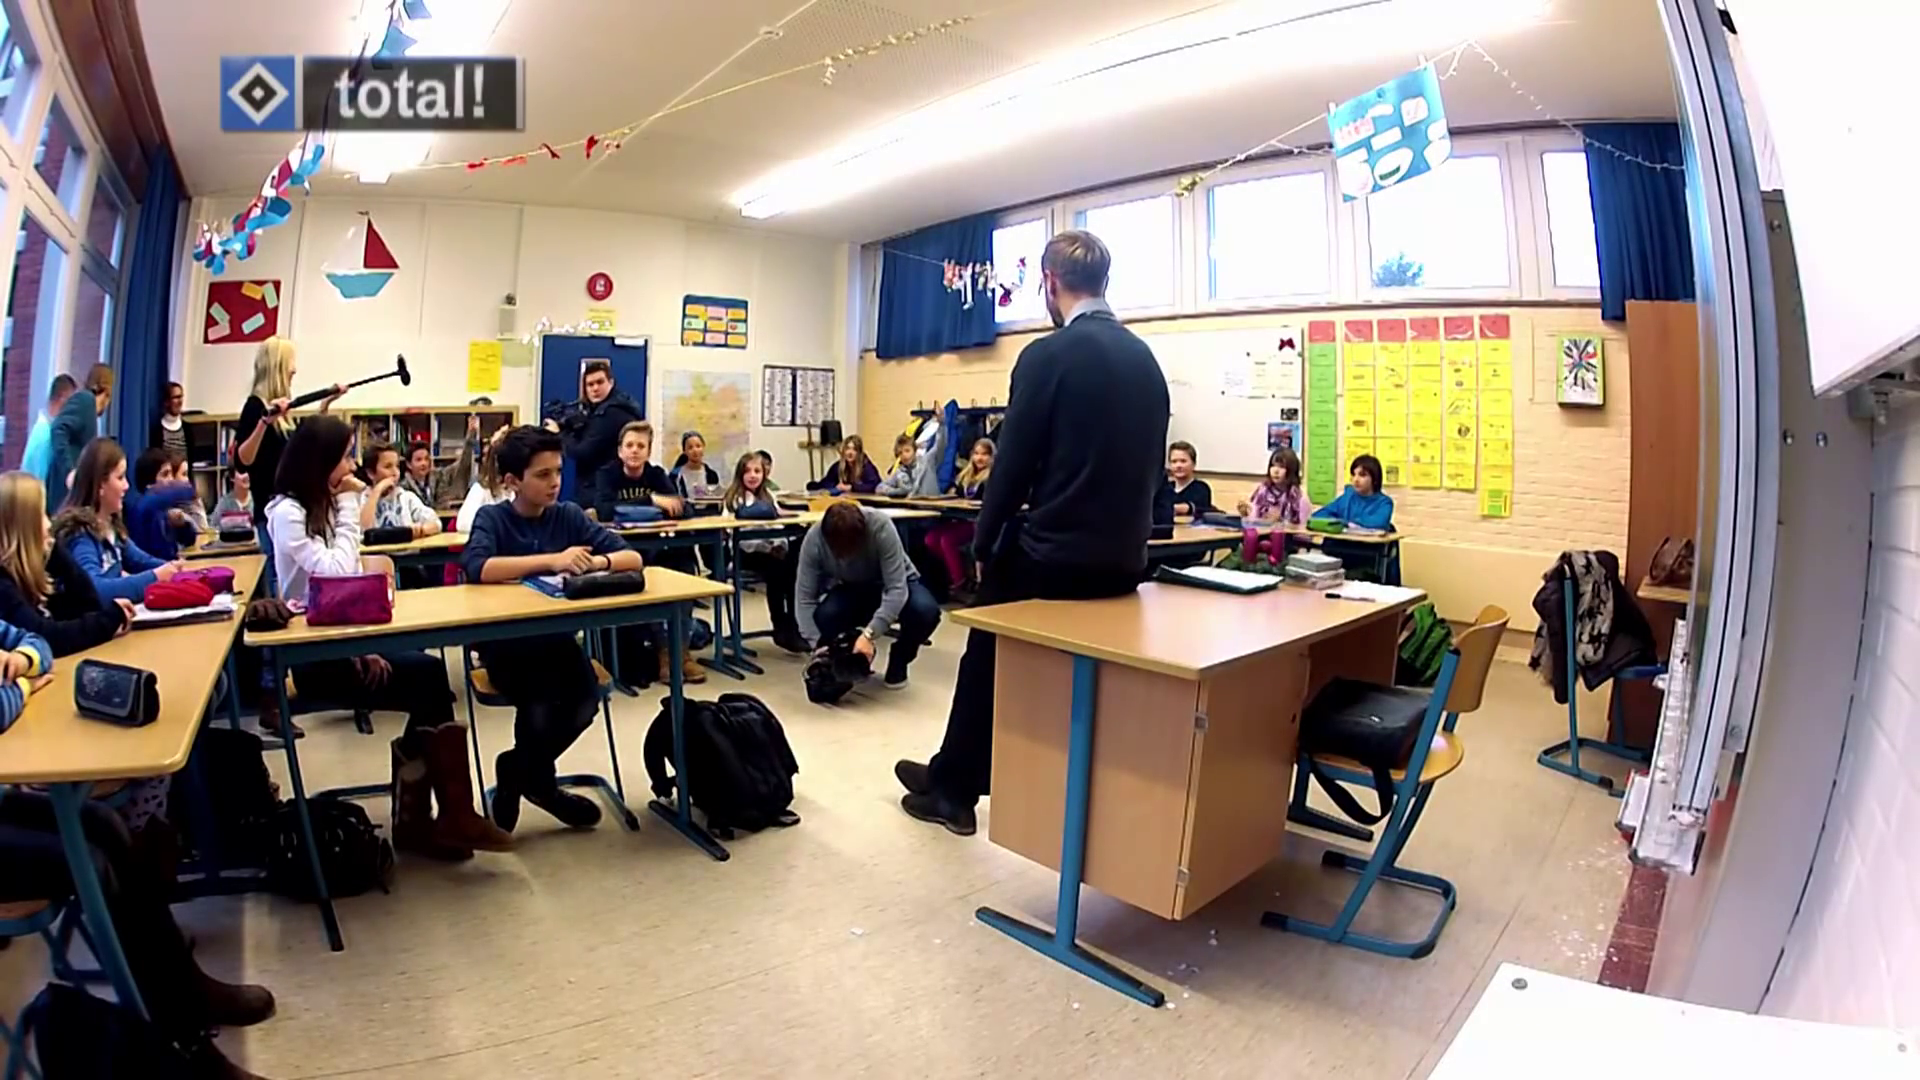
\includegraphics[width=0.8\linewidth]{img/Schulklasse}
	\caption{Eine Screenshot des YouTube-Videos \glqq Maxi Beister als Herr Müller überrascht eine Schulklasse\grqq \cite{Schulklasse_Video}}
	\label{fig:schulklasse}
\end{figure}
